\documentclass[a4paper, 11pt]{article}
\usepackage{comment}  
\usepackage{lipsum} 
\usepackage{fullpage} 
\usepackage[table]{xcolor}%
\usepackage{graphicx}

\begin{document}

\noindent
\large\textbf{ASCI/AGRO 931} \hfill \textbf{Name: Gerardo Mamani} \\
\normalsize Homework 4 (25 pts) \hfill  \\
Due Friday, Oct 13, at the beginning of class \hfill 
Show your work! \hfill

\begin{enumerate}

\item (15 points) Below is the pedigree of Roan Gauntlet, an English bull. Rectangles indicate bulls and ovals indicate cows. All mates not included in the pedigree are outside the family tree and therefore assumed to be unrelated. Note: Lord Raglan was mated to three different dams to produce the three offspring in the figure. \\

\begin{figure}[h]
    \centering
    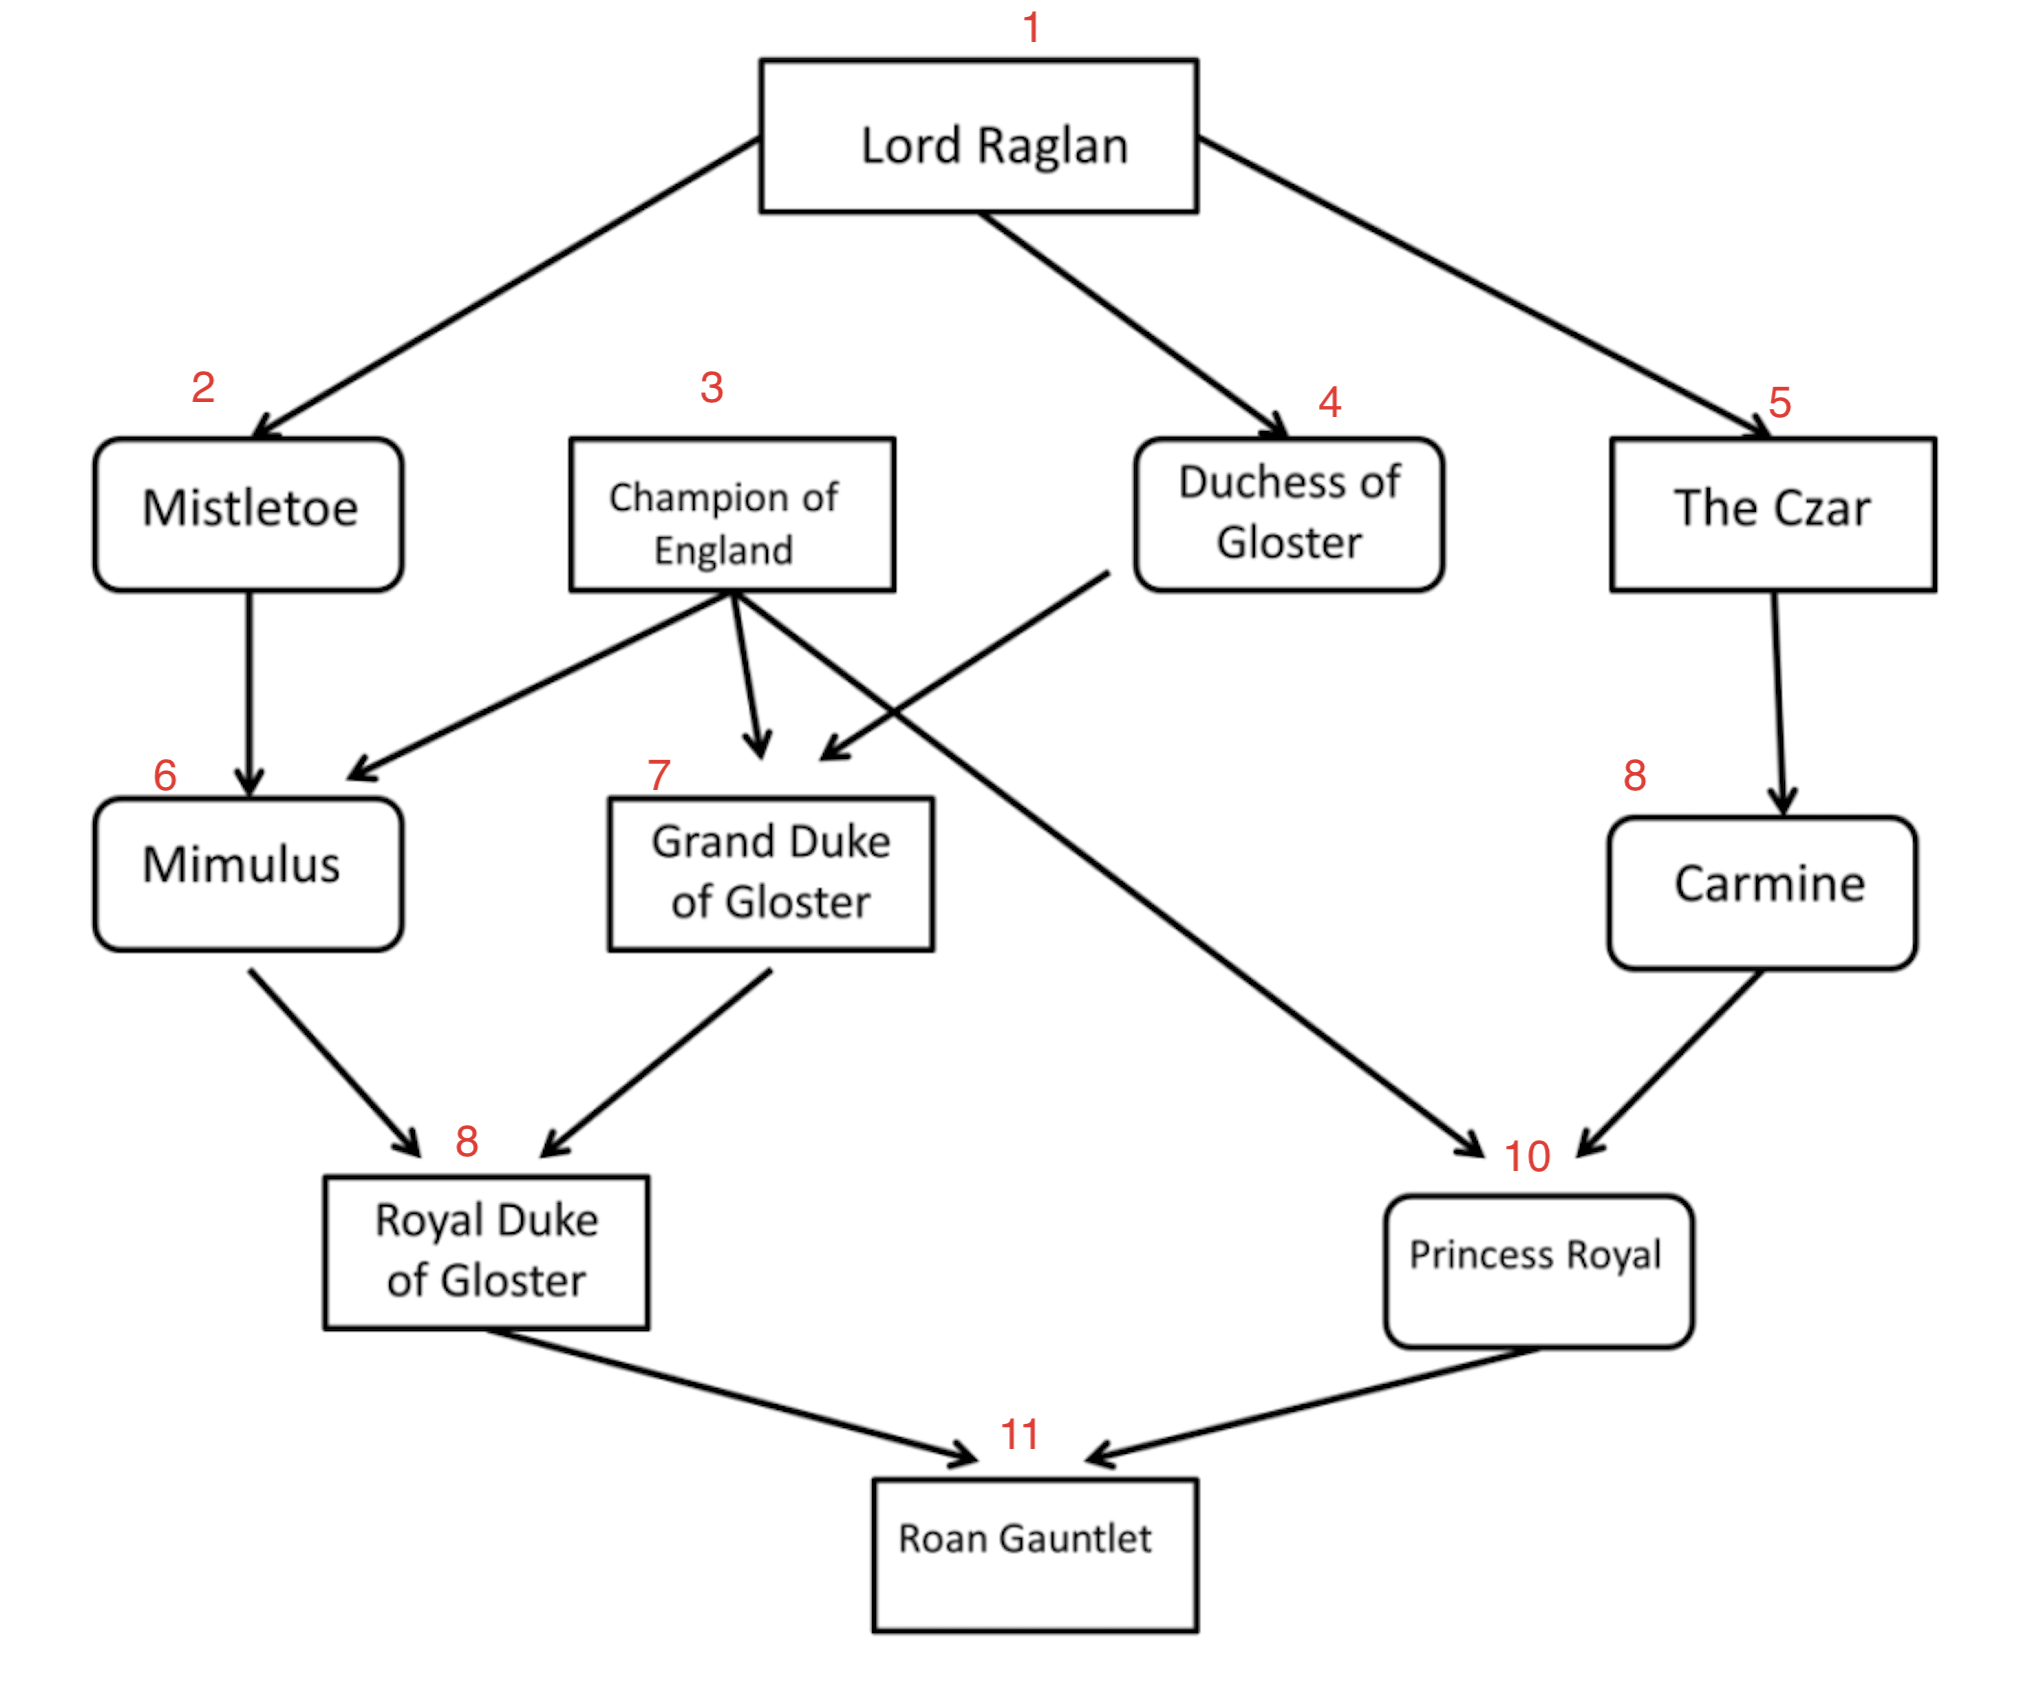
\includegraphics[height=0.5\textwidth]{Homework4_pedigree.png}
    \caption{Pedigree of Roan Gauntlet}
\end{figure}

\subitem a. Calculate the inbreeding coefficients for Royal Duke of Gloster, Princess Royal, and Roan Gauntlet.

\begin{itemize}
\item Paths for $F_{Royal Duke of Gloaster} = F_{9}$\\

- 6 2 \textbf{1} 4 7 = \[(\frac{1}{2})^5 = \frac{1}{32}\] \\
- 6 \textbf{3} 7 = \[(\frac{1}{2})^3 = \frac{1}{8}\]\\
Then \[F_{Royal Duke of Gloaster} = \frac{1}{32} + \frac{1}{8} = 0.15625 \] \\

\item Paths for $F_{Princess Royal} = F_{10}$\\

Don't have paths\\

\item Paths for $F_{Roan Gauntlet} = F_{11}$\\

- 2 6 9  \textbf{1} 10 8 5  = \[(\frac{1}{2})^7 = \frac{1}{128}\] \\
- 9 6 \textbf{3} 10 = \[(\frac{1}{2})^4 = \frac{1}{16}\]\\
- 9 7 4  \textbf{1} 5 8 10 = \[(\frac{1}{2})^7 = \frac{1}{128}\]\\
- 9 7 \textbf{3} 10 = \[(\frac{1}{2})^4 = \frac{1}{16}\]\\
Then \[F_{Roan Gauntlet} = \frac{1}{128} + \frac{1}{16}+ \frac{1}{128}+ \frac{1}{16} = 0.140625 \]\\

\end{itemize}

\subitem b. Produce a table of coefficients of co-ancestry for all individuals in the first three generations only (everyone except for Royal Duke of Gloster, Princess Royal, and Roan Gauntlet. Do not include mates not shown in the diagram. (hint: the tabular method may be useful here)

\begin{itemize}
\item By tabular method we have the additive or numerator relationship matrix \(a_{xy}\) :

\begin{tabular}{|c|c|c|c|c|c|c|c|c|}
\hline
	&	1      	&	2     	&	3	      &	4	      &	5	      &	6      	&	7     	&	8 \\ \hline
1	&	1.0000	&	0.5000	&	0.0000	&	0.5000	&	0.5000	&	0.25000	&	0.25000	&	0.25000 \\ \hline
2	&	0.5000	&	1.0000	&	0.0000	&	0.2500	&	0.2500	&	0.50000	&	0.12500	&	0.12500 \\ \hline
3	&	0.0000	&	0.0000	&	1.0000	&	0.0000	&	0.0000	&	0.50000	&	0.50000	&	0.00000 \\ \hline
4	&	0.5000	&	0.2500	&	0.0000	&	1.0000	&	0.2500	&	0.12500	&	0.50000	&	0.12500 \\ \hline
5	&	0.5000	&	0.2500	&	0.0000	&	0.2500	&	1.0000	&	0.12500	&	0.12500	&	0.50000 \\ \hline
6	&	0.2500	&	0.5000	&	0.5000	&	0.1250	&	0.1250	&	1.00000	&	0.31250	&	0.06250 \\ \hline
7	&	0.2500	&	0.1250	&	0.5000	&	0.5000	&	0.1250	&	0.31250	&	1.00000	&	0.06250 \\ \hline
8	&	0.2500	&	0.1250	&	0.0000	&	0.1250	&	0.5000	&	0.06250	&	0.06250	&	1.00000 \\ \hline
\end{tabular}
\\\\
\item The additive or numerator relationship matrix (\(a_{xy}\)) is twice the coancestry (\(r_{xy}\)). Then dividing by 2, we have the next matrix of coancestry:

\begin{tabular}{|c|c|c|c|c|c|c|c|c|}
\hline
	&	1	&	2	&	3	&	4	&	5	&	6	&	7	&	8 \\ \hline
1	&	0.5000	&	0.2500	&	0.0000	&	0.2500	&	0.2500	&	0.1250	&	0.1250	&	0.1250 \\ \hline
2	&	0.2500	&	0.5000	&	0.0000	&	0.1250	&	0.1250	&	0.2500	&	0.0625	&	0.0625 \\ \hline
3	&	0.0000	&	0.0000	&	0.5000	&	0.0000	&	0.0000	&	0.2500	&	0.2500	&	0.0000 \\ \hline
4	&	0.2500	&	0.1250	&	0.0000	&	0.5000	&	0.1250	&	0.0625	&	0.2500	&	0.0625 \\ \hline
5	&	0.2500	&	0.1250	&	0.0000	&	0.1250	&	0.5000	&	0.0625	&	0.0625	&	0.2500 \\ \hline
6	&	0.1250	&	0.2500	&	0.2500	&	0.0625	&	0.0625	&	0.5000	&	0.1563	&	0.0313 \\ \hline
7	&	0.1250	&	0.0625	&	0.2500	&	0.2500	&	0.0625	&	0.1563	&	0.5000	&	0.0313 \\ \hline
8	&	0.1250	&	0.0625	&	0.0000	&	0.0625	&	0.2500	&	0.0313	&	0.0313	&	0.5000 \\ \hline
\end{tabular}
\end{itemize}

\item (4 pts) Fill in the blanks: Coancestry of an individual with his/herself is \textbf{\((1+F_{i})/2 = 0.5\)} and is equal to the level of inbreeding observed after \textbf{1} generation(s) of self-fertilization (assume no inbreeding in the founding individual).

\item (6 pts) Consider a 4-generation pedigree. Progeny E is the product of a full-sib mating between individuals C and D. C and D are both progeny of founders, A and B. How much does the inbreeding of individual E increase if the parents of individual B are full-siblings relative to that if they (the parents of B) are unrelated?

\begin{figure}[!h]
    \centering
    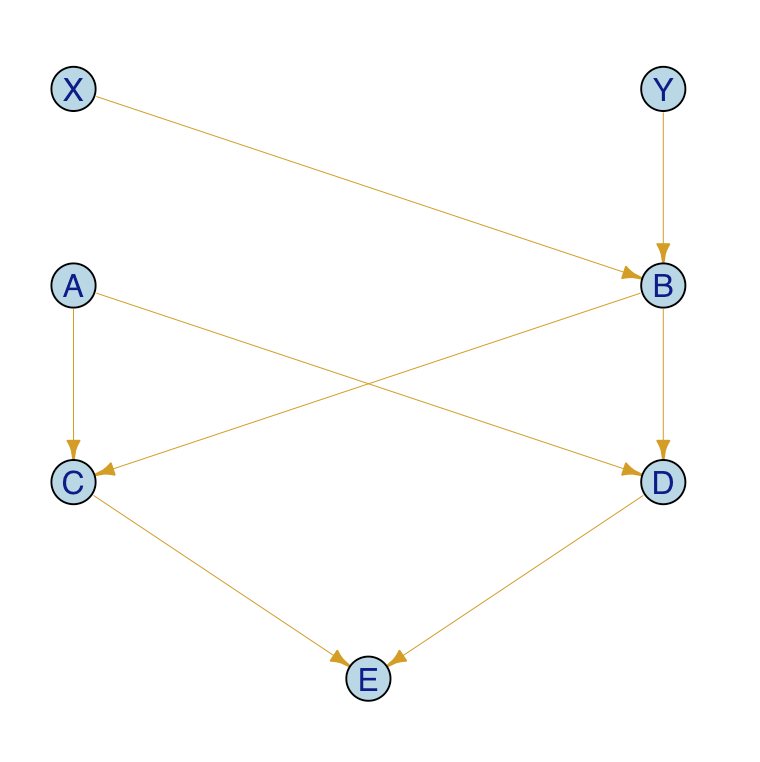
\includegraphics[height=0.5\textwidth]{Homework4a.png}
    \caption{ Pedigree parents of B unrelated}
\end{figure}

\begin{itemize}
\item Paths for $F_{E}$\\

- C \textbf{B} D = \[(\frac{1}{2})^3(1+F_B) = (\frac{1}{2})^3(1+0)=\frac{1}{8}\] \\
- C \textbf{A} D = \[(\frac{1}{2})^3(1+F_A) = (\frac{1}{2})^3(1+0)=\frac{1}{8}\] \\
Then \[F_{E} = \frac{1}{8} + \frac{1}{8} = 0.25 \] \\
\end{itemize}

\newpage

\begin{figure}[h]
    \centering
    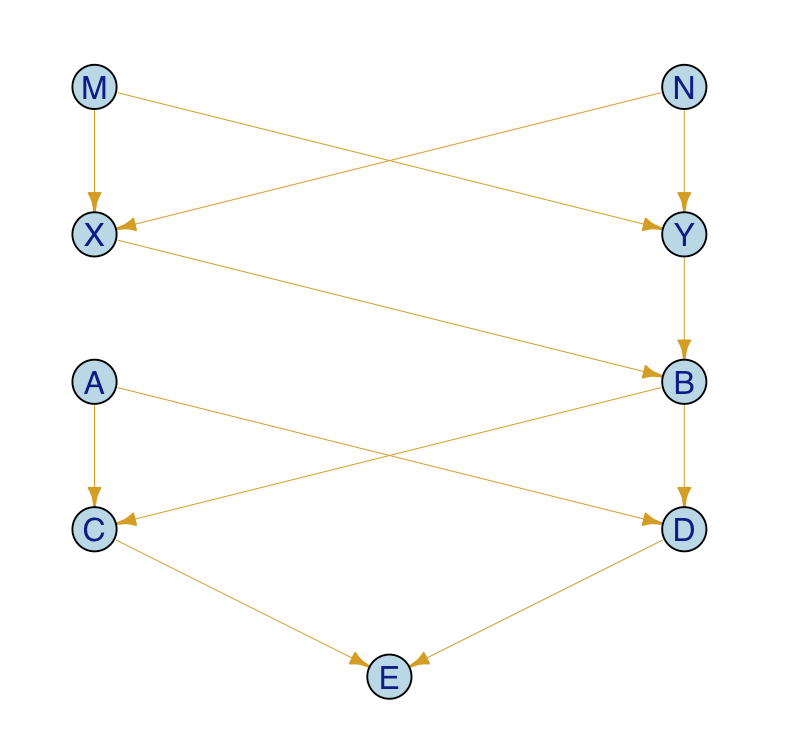
\includegraphics[height=0.5\textwidth]{Homework4b.png}
    \caption{ Pedigree parents of B are related}
\end{figure}

\begin{itemize}

\item If X and Y are full-sibling then the paths for \(F_B\)

- X \textbf{M} Y = \[(\frac{1}{2})^3(1+F_M) = (\frac{1}{2})^3(1+0)=\frac{1}{8}\] \\
- X \textbf{N} Y = \[(\frac{1}{2})^3(1+F_N) = (\frac{1}{2})^3(1+0)=\frac{1}{8}\] \\
Then \[F_{B} = \frac{1}{8} + \frac{1}{8} = \frac{1}{4} \] \\

\item Paths for $F_{E}$\\

- C \textbf{B} D = \[(\frac{1}{2})^3(1+F_B) = (\frac{1}{2})^3(1+\frac{1}{4})=\frac{5}{32}\] \\
- C \textbf{A} D = \[(\frac{1}{2})^3(1+F_A) = (\frac{1}{2})^3(1+0)=\frac{1}{8}\] \\
Then \[F_{E} = \frac{5}{32} + \frac{1}{8} = 0.28125 \] \\

\(0.28125 - 0.25 = \textbf{0.03125}\)

\end{itemize}
\end{enumerate}

\end{document}
